% !TEX TS-program = xelatex
% !TEX encoding = UTF-8 Unicode
% !Mode:: "TeX:UTF-8"

\documentclass{resume}
\usepackage{zh_CN-Adobefonts_external} % Simplified Chinese Support using external fonts (./fonts/zh_CN-Adobe/)
%\usepackage{zh_CN-Adobefonts_internal} % Simplified Chinese Support using system fonts
\usepackage{linespacing_fix} % disable extra space before next section
\usepackage{cite}
\usepackage{graphicx}
\usepackage{tabu}
\usepackage{multirow}
\begin{document}
\pagenumbering{gobble} % suppress displaying page number


%\name{谈啸}

%{E-mail}{mobilephone}{homepage}
% be careful of _ in emaill address
%\contactInfo
%{\faPhone\ (+86) 189-1285-6482}{\faEnvelope\ haiantanxiao@gmail.com}{\faInternetExplorer\ http://xiaotan.tech}{\faInfoCircle\ 江苏南通}{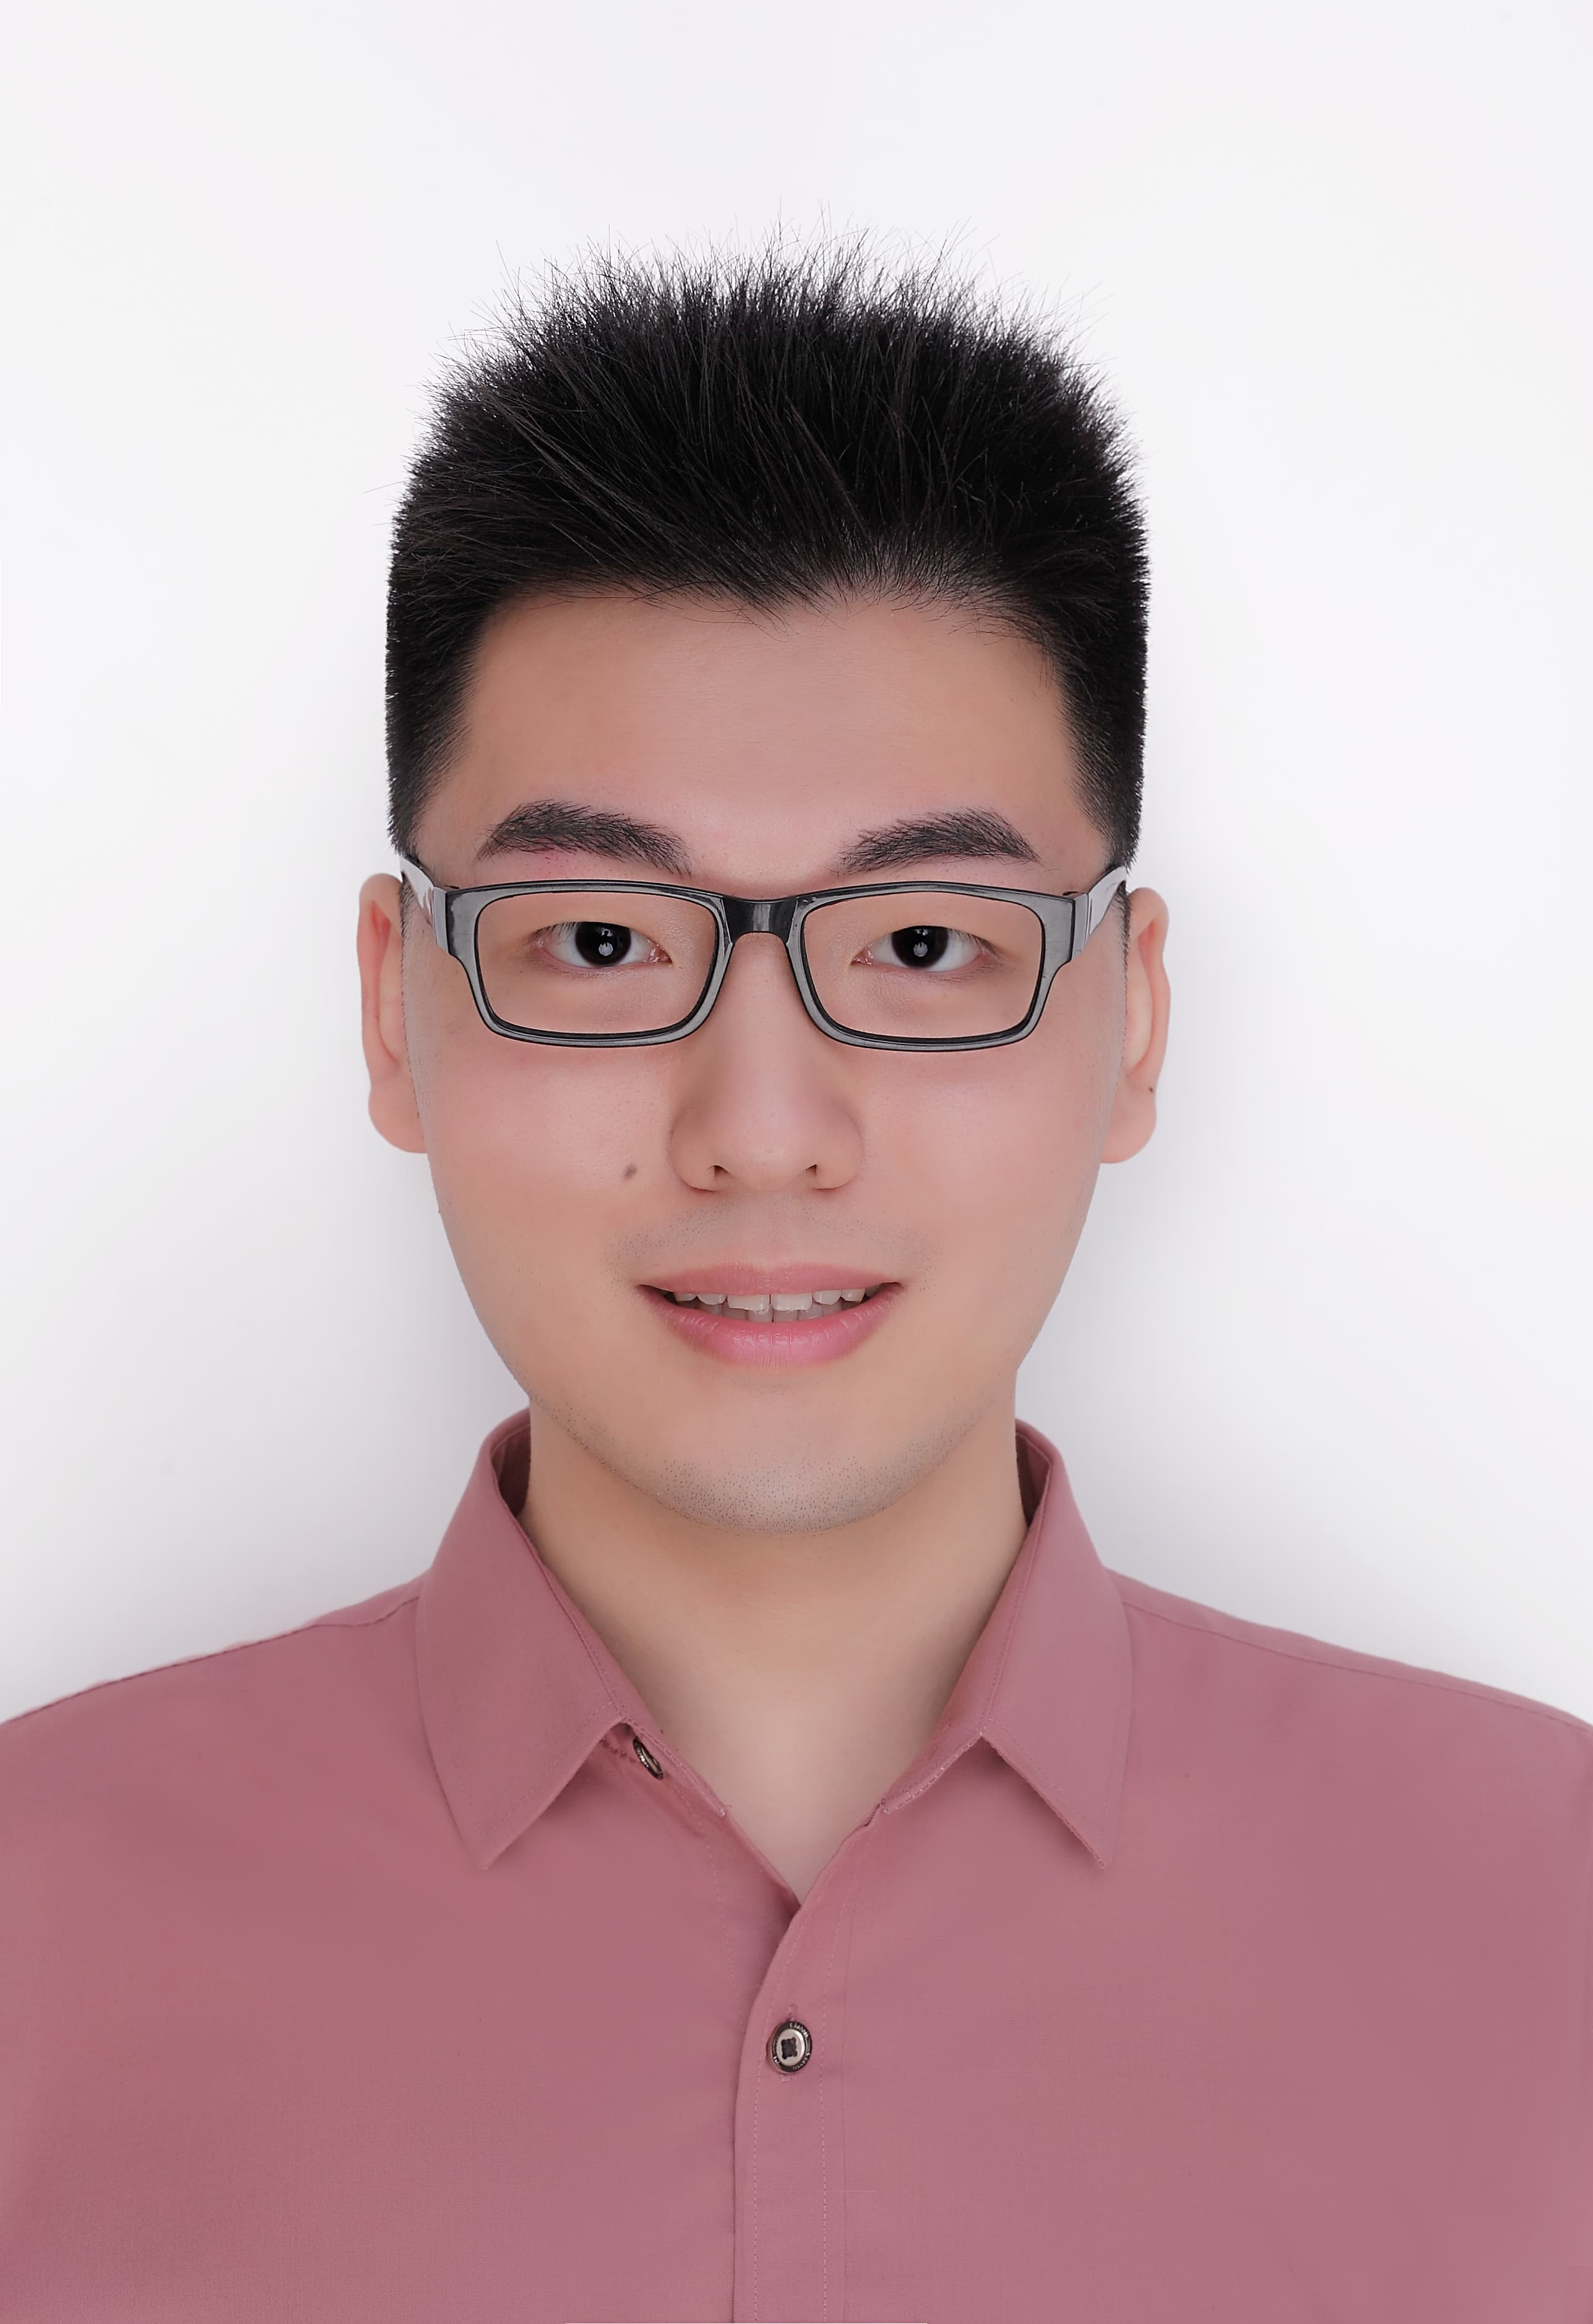
\includegraphics[width=0.88in]{photo.jpg}}{}


% change Large font here
\Large{
  \begin{tabu}{ c l l}
   \multirow{5}{1in}{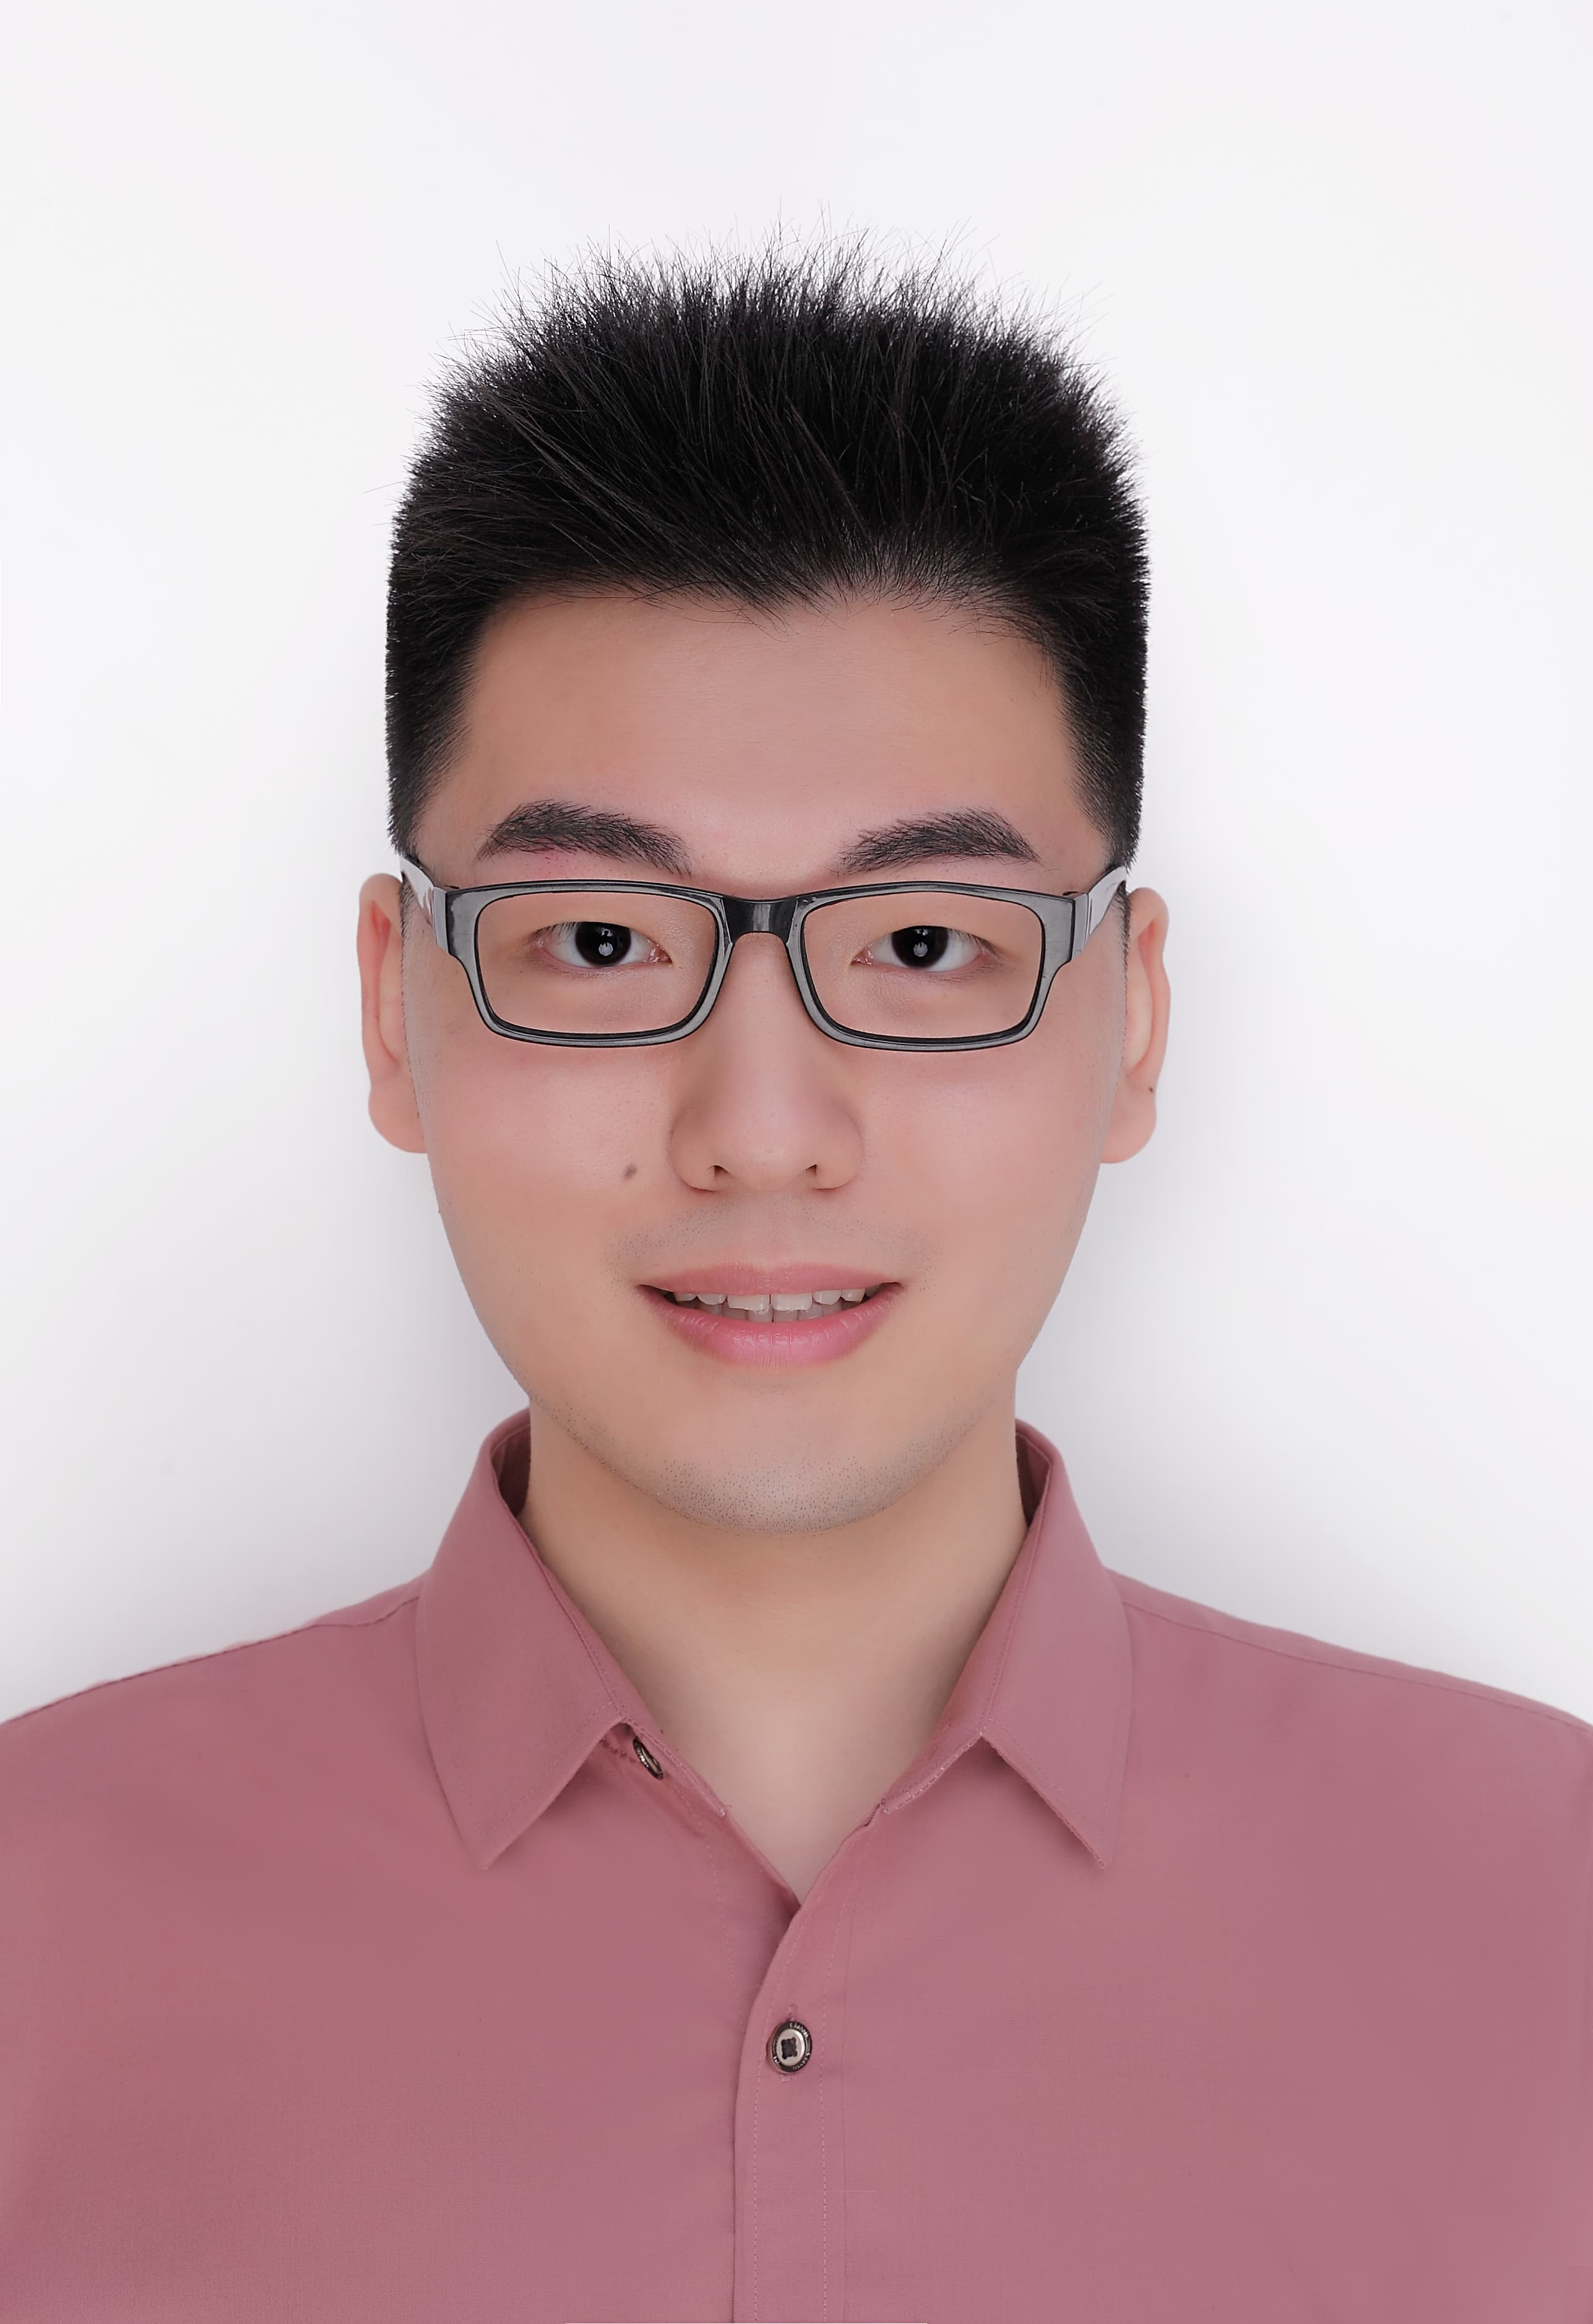
\includegraphics[width=0.9in]{photo.jpg}}\\ 
    & \huge{\scshape{谈啸}}\\
    & \faPhone\ (+86) 189-1285-6482
    & \faEnvelope\ theo.tan@hotmail.com\\
    & \faInternetExplorer\ http://xiaotan.tech
    & \faWeixin\ tanxiao\_js\\
    & \faLinkedin\ linkedin.com/in/tan-xiao
    & \faGithub\ github.com/WHU-Tan\\
  \end{tabu}
}

% {E-mail}{mobilephone}
% keep the last empty braces!
%\contactInfo{xxx@yuanbin.me}{(+86) 131-221-87xxx}{}

 
%\section{\faHeartO\ 个人总结}
%\par 我自认是一个不容易沉心来,在某个领域成为顶尖专才的人,更希望什么百科知识都能懂一些,交叉学科的发展对我而言有着迷人的魅力,因此,无论是法学双学位的修读,还是商科相关项目与实习经历的参与,都是我将各领域知识进行融合应用的表现。
%\par 同时,我也知道自己是一个喜欢刺激大脑来寻找快感的人,因此,我积极参加学生工作与志愿活动,以极高的工作热情与较强的领导能力面对每一个未曾涉足的领域,结识每一种形形色色的人群。
%\par 本科期间的国际交流与即将攻读的海外硕士学位,让我不仅掌握两种语言,两种文化,有两套操作系统,使我不仅仅是个双语人,更是个双文化人,有两个可以随时切换的文化体系。


\section{\faGraduationCap\ 教育背景}
%\section{教育背景}
\datedsubsection{\textbf{武汉大学电子信息学院},电子信息工程,\textit{教育部``卓越工程师培养计划''试点班}}{2017.9 - 至今}
\normalsize{
\begin{itemize}
  \item 核心课程: 高等数学(92)、线性代数(98)、数字信号处理(92)、人工智能进展(93)、项目管理(90)、商业运营模拟(95)等
  \item \textbf{连续两年}获武汉大学优秀学生干部;武汉大学优秀青年志愿者
  \item 获武汉大学乙等奖学金\textbf{(综合排名前15\%)};赴新加坡国立大学参加\textbf{人工智能与商业管理}课程
\end{itemize}
}

\datedsubsection{\textbf{武汉大学法学院},法学,\textit{法学双学位}}{2019.1 - 至今}
\begin{itemize}
    \item 核心课程: 宪法(93)、行政法(95)、民法、经济法、国际经济法等
    \item 领导知识产权保护与开源软件传统冲突专题研究小组并写作论文
\end{itemize}

% \end{itemize}

\section{\faUsers\ 项目/实习经历}
% increase linespacing [parsep=0.5ex]
\datedsubsection{基于用户身体素质的食疗推荐系统, \textbf{项目发起人}}{2020年3月-至今}
\begin{itemize}
    \item 基于深度学习和知识图谱技术,通过面部图片和问卷判断体质,通过食疗推荐帮助用户改善体质
    \item 作为\textbf{项目创始人},负责项目\textbf{市场分析、财务分析与融资计划}的构建,\textbf{统筹商业计划书的写作},专利文档的写作与微信小程序的开发
\end{itemize}
\datedsubsection{\textbf{基于可信区块链溯源的动力电池评估与回收平台}, 项目创始人}{2019年4月-至今}
\begin{itemize}
    \item 基于\textbf{自主研发}的公有链everiToken,利用RFID作为终端信息交互设备,提供动力电池全生命周期的\textbf{监管与回收}服务
    \item \textbf{项目创始人},负责项目\textbf{技术架构}的构建,\textbf{专利文档}的修改,参与\textbf{EI检索论文}的写作
    \item \textbf{与宇链科技对接},将自研公有链everiToken\textbf{落地应用};对动力电池回收市场进行研究并制作\textbf{行研报告}
    \item 项目曾获2019年``花旗杯''金融创新应用大赛\textbf{全国五强},武汉大学第十届``自强杯''创业大赛一等奖
\end{itemize}

\datedsubsection{\textbf{基于数据智能的中国大学生抑郁疏导对话机器人的研究与实现}, 技术组组长}{2018年9月-至今}
\begin{itemize}
    \item \textbf{国家级}大学生科研项目
    \item 分析中国大学生\textbf{心理认知结构},构建抑郁疏导模型与抑郁疏导领域的\textbf{知识图谱},实现基于抑郁疏导模型的机器人对话策略
    \item 负责基于知识图谱,通过结巴分词,规则匹配将相应的\textbf{自然语言转换成SPARQL}查询语句,搭建具有逻辑推理能力与上下文一致性的\textbf{对话机器人}
\end{itemize}

\datedsubsection{\textbf{基于FPGA的前列腺增生双极电切手术AI预警系统}, 执行组组长}{2018年6月-2019年9月}
\begin{itemize}
    \item 借助图像识别、深度学习等技术,\textbf{国内首次}在FPGA硬件平台上搭建基于卷积神经网络的前列腺增生双极电切手术AI预警系统,并借助FPGA硬件特性实现卷积神经网络的运算加速
    \item 负责利用\textbf{生成式对抗网络(GAN)}对数据集进行增强,对比系统与PC端、嵌入式设备性能
    \item 负责\textbf{统筹作品书(100页)的写作}、进行项目的\textbf{市场分析、商业模式构建、风险控制分析}
    \item 项目曾获\textbf{第十六届``挑战杯''全国大学生课外学术科技作品竞赛三等奖},湖北省``挑战杯''一等奖,武汉大学``自强杯''特等奖;获中美青年创客大赛(湖北赛区)二等奖
\end{itemize}

\datedsubsection{\textbf{天津市南开区政府合作交流办公室}, 工作助理}{2019年8月}
\begin{itemize}
    \item 作为武汉大学代表\textbf{(本科生共5人)}入选南开区委组织部\textbf{``云帆计划''}人才引进计划
    \item 与对口支援扶贫干部进行对接,对扶贫专项资金的使用情况进行核对,\textbf{编写VBA批处理程序}提高工作效率
    \item 为办公室撰写工作经验分享两篇,均\textbf{刊登于南开区委内部刊物}
\end{itemize}
\datedsubsection{\textbf{容诚会计师事务所(南京分所)}, 审计部门助理}{2020年1月-2020年3月}
\begin{itemize}
    \item 参与检查公司账面数据,完成\textbf{账目盘点和现金盘查},找出\textbf{三处}不合规之处
    \item 汇总近\textbf{五十个财务模块数据},编制下半年财务规划,分析项目成本重大资金费用内部驱动因素,对其进行分析、控制
\end{itemize}

\section{\faTrophy\ 竞赛获奖}
 \datedsubsection{\textbf{第十六届``挑战杯''全国大学生课外学术科技作品竞赛}, 三等奖}{2019年9月}
\begin{itemize}
  \item \textit{前列腺增生双极电切手术AI预警及远程专家辅助系统}
  \item 负责进行\textbf{项目的全部路演},全环节的\textbf{竞赛事务跟进处理}%:与设计师沟通作品书与海报的排版,与影视公司商榷演示视频的制作,与承办方确认场地的细节,并且与校、省、团中央三级的竞赛负责人沟通
\end{itemize}

\datedsubsection{\textbf{2020年美国大学生数学建模竞赛(MCM)},优异(一等)奖(Meritorious),\textbf{全球前7\%}}{2020年3月}
\begin{itemize}
  \item \textit{Feedback and Review: Consumers and Content Creators Centric Mechanism}%(反馈与评论:消费者与评论贡献者为中心的机制)
  \item 通过对\textbf{用户画像}的绘制、评论文本的\textbf{情感分析}、打分分值的\textbf{回归分析},分析吹风机、微波炉、奶嘴等产品的用户满意度、历史销量与购买关联度等信息,为平台经理提出改善建议
  \item 负责团队沟通、数据清洗(pandas, numpy)、自然语言处理(LSTM)、\textbf{数据可视化}(PowerBI, MATLAB)、英文论文(共17页)写作与LaTeX排版
 \end{itemize}
 
 \datedsubsection{\textbf{2019年``花旗杯''金融创新应用大赛},全国五强}{2019年11月}
 \begin{itemize}
   \item \textit{PBChain——基于可信区块链溯源的动力电池评估与回收平台}
   \item 花旗银行发起\textbf{FinTech竞赛},重点考察信息科技在金融业的应用
   \item 负责\textbf{全英文演示文稿制作与路演讲稿写作},\textbf{作为队长参与答辩},与花旗银行进行事务沟通
 \end{itemize}

\section{\faBook\ 专利/论文}
\begin{itemize}[parsep=0.2ex]
  \item 发明专利:一种基于可信区块链的动力电池溯源方法, \textit{201910140955.X}
  \item 发明专利:一种基于可信区块链的动力电池追踪定位的系统及方法, \textit{201910140942.X}
  \item 实用新型专利:一种基于个人身体素质的食疗推荐装置
  \item \textbf{EI检索}论文:Evaluation and recovery of power batteries based on trusted blockchain traceability, \textit{IOP Conference Series: Materials Science and Engineering}
  \item 教材附录: 基于Nexys A7的贪吃蛇游戏的设计与实现, \textit{《RISC-V:基础与实践》}, 清华大学出版社
\end{itemize}


% \begin{onehalfspacing}
% \end{onehalfspacing}

% \datedsubsection{\textbf{DID-ACTE} 荷兰莱顿}{2015年3月 - 2015年6月}
% \role{本科毕业设计}{LIACS 交换生}
% 利用结巴分词对中国古文进行分词与词性标注,用已有领域知识训练形成 classifier 并对结果进行调优
% \begin{onehalfspacing}
% \begin{itemize}
%   \item 利用结巴分词对中国古文进行分词与词性标注
%   \item 利用已有领域知识训练形成 classifier, 并用分词结果进行测试反馈
%   \item 尝试不同规则,对 classifier 进行调优
% \end{itemize}
% \end{onehalfspacing}


% \section{\faHeartO\ 项目/作品摘要}
% \section{项目/作品摘要}
% \datedline{\textit{An Integrated Version of Security Monitor Vis System}, https://hijiangtao.github.io/ss-vis-component/ }{}
% \datedline{\textit{Dark-Tech}, https://github.com/hijiangtao/dark-tech/ }{}
% \datedline{\textit{融合社交网络数据挖掘的电视节目可视化分析系统}, https://hijiangtao.github.io/variety-show-hot-spot-vis/}{}
% \datedline{\textit{LeetCodeOJ Solutions}, https://github.com/hijiangtao/LeetCodeOJ}{}
% \datedline{\textit{Info-Vis}, https://github.com/ISCAS-VIS/infovis-ucas}{}


\section{\faSlideshare\ 学生工作经历}
%\section{社区参与/实践}
% increase linespacing [parsep=0.5ex]
\datedsubsection{\textbf{武汉大学党委学生工作部新媒体中心}, 总负责人}{2018.9-至今}
\begin{itemize}
  \item \textbf{中心创始人},注册运营``武汉大学学生工作部''微信公众号,一年内关注人数\textbf{由零突破一万}
  \item \textbf{带领近三十人团队},参与``开学第一课''校长讲座、``榜样珞珈''颁奖典礼等活动的现场统筹
  \item 为中心微信公众号\textbf{撰稿、剪辑视频},两次\textbf{阅读量破五万}
\end{itemize}

\datedsubsection{\textbf{武汉大学青年志愿者协会行政办公室}, 部委、副部}{2017.9-2019.6}
\begin{itemize}
  \item 参与组织校青年志愿者大会、校``公益嘉年华''、校优秀志愿项目评比,参与人次\textbf{近万次}
  \item 所对接项目获中国青年志愿服务项目大赛特等奖、阿克苏诺贝尔中国大学生社会公益奖金奖
\end{itemize}

\datedsubsection{\textbf{武汉大学自强Studio},部委}{2017.9-2018.6}
\begin{itemize}
  \item 参与策划``奔跑吧珞珈''、``十大珞珈风云学子''等校园品牌活动,\textbf{参与人数近四万次}
  \item 运营学生评课系统``淘课啦'',以后台数据为基础,运用LDA模型\textbf{分析评论文本},高斯分布模型\textbf{老师口碑},得出结论并撰写推文《这些课程最受武大学子欢迎》,\textbf{获得10万阅读量}
\end{itemize}


%\section{\faCogs\ IT 技能}
% increase linespacing [parsep=0.5ex]
%\begin{itemize}[parsep=0.2ex]
%  \item \textbf{编程语言、操作系统与工程构建: }Python, MATLAB, C, C$\#$, Verilog; Linux, Git, AWS
%  \item \textbf{效率工具: }LaTeX, PowerBI, Excel; Pr, AE
%\end{itemize}

\section{\faHeartO\ 技能/特长爱好}
\begin{itemize}
  \item \textbf{编程语言、操作系统与工程构建: }Python, MATLAB, C, C$\#$, Verilog; Linux, Git 
  \item \textbf{效率工具: }LaTeX, PowerBI, Excel; Pr, AE
  \item \textbf{语言技能: }CET-6(612), TOEFL94;中西部翻译大赛(湖北赛区)笔译二等奖、口译三等奖
  \item \textbf{爱好特长: }热心公益,累计参加志愿者活动25次:英国前首相特蕾莎梅访华接待志愿者,``武汉台湾周''中国国民党前主席洪秀柱来访接待志愿者,``世界女大学校长论坛''志愿者,武汉网球公开赛优秀志愿者等;主持撰稿:担任校青年志愿者协会迎新活动、武汉大学十大志愿项目评比等活动主持人
\end{itemize}


%% Reference
%\newpage
%\bibliographystyle{IEEETran}
%\bibliography{mycite}
\end{document}
